\begin{frame}
\frametitle{Outline of the presentation}
\begin{itemize}
	\item \color{mygray} Expected exit time from a domain
	\begin{itemize} \color{mygray}
		\item[--] Setting
		\item[--] Numerical methods
		\item[--] Numerical experiments
	\end{itemize} 
	\item Theoretical investigation: perturbed SDE's \color{black}
	\item The uncertain Darcy's problem 
\end{itemize}
\end{frame}

\begin{frame}
\frametitle{Darcy's problem - Setting}
Consider 
\begin{equation*}
	\left \{
  	\begin{aligned}
		u &= -A \nabla p, && \text{in } D, \\
		\nabla\cdot u &= 0, && \text{in } D, \\
		p &= p_0, && \text{on } \Gamma_{in},\\
		p &= 0, && \text{on } \Gamma_{out}, \\
		\nabla p \cdot n &= 0, && \text{on } \Gamma_N,
	\end{aligned} \right.
\end{equation*}
where $A$ is a random field such that $A = e^\gamma$, where 
\begin{equation*}
	\mathrm{cov}_\gamma(x_1,x_2) = \frac{\sigma_A^2}{\Gamma(\nu)2^{\nu-1}}\Big(\sqrt{2\nu}\frac{|x_1-x_2|}{L_c}\Big)^\nu K_{\nu}\Big(\sqrt{2\nu}\frac{|x_1-x_2|}{L_c}\Big), 
\end{equation*}
for $\nu \geq 0.5$. For each realization of $A$, we solve the equation with linear FEM on a regular grid with \texttt{FreeFem++}.
\end{frame}

\begin{frame}
\frametitle{A realization of the solution}
\begin{figure}[t]
    \centering
    \begin{subfigure}{0.49\linewidth}
        \centering
	\includegraphics[width=4.5cm,height=3cm]{Pictures/A.jpg}
        \caption{Random field}
    \end{subfigure}
    \begin{subfigure}{0.49\linewidth}
        \centering
	\includegraphics[width=4.5cm,height=3cm]{Pictures/P.jpg}
        \caption{Pressure}
    \end{subfigure}
    \begin{subfigure}{0.49\linewidth}
        \centering
	\includegraphics[width=4.5cm,height=3cm]{Pictures/Ux.jpg}
        \caption{$x$ component of velocity field}
    \end{subfigure}
    \begin{subfigure}{0.49\linewidth}
        \centering
	\includegraphics[width=4.5cm,height=3cm]{Pictures/Uy.jpg}
        \caption{$y$ component of velocity field}
    \end{subfigure} 
\end{figure}
\end{frame}

\begin{frame}
\frametitle{Darcy's solution in DEM and CEM}
Evaluation of the FEM solution at each time step \\ $\to$ unaffordable computational cost

\vspace{0.5cm}
\begin{minipage}[0]{0.49\linewidth}
	\centering
	\resizebox{1\linewidth}{!}{% This file was created by matlab2tikz.
%
%The latest updates can be retrieved from
%  http://www.mathworks.com/matlabcentral/fileexchange/22022-matlab2tikz-matlab2tikz
%where you can also make suggestions and rate matlab2tikz.
%
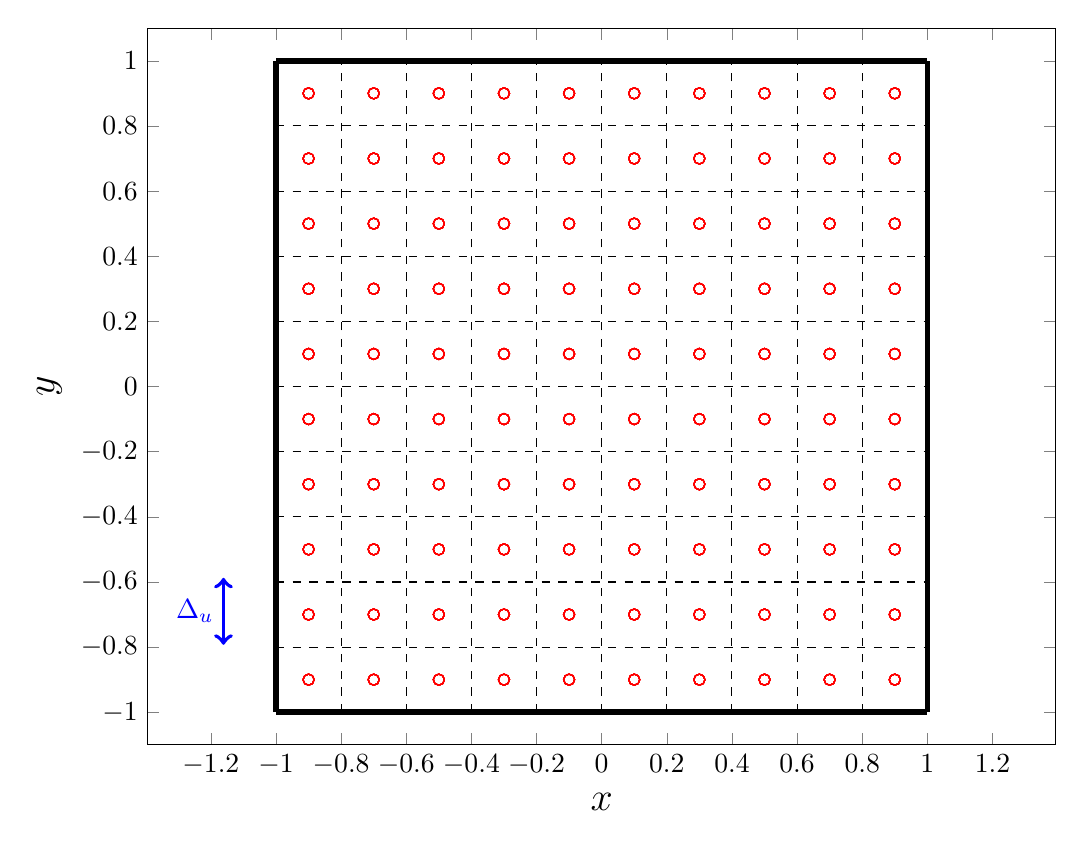
\begin{tikzpicture}



\begin{axis}[%
width=4.542in,
height=3.583in,
at={(0.801in,0.484in)},
scale only axis,
xmin=-1.39468302658487,
xmax=1.39468302658487,
xlabel={$x$},
xlabel style={font=\Large},
ymin=-1.1,
ymax=1.1,
ylabel={$y$},
ylabel style={font=\Large},
axis background/.style={fill=white}
]
\addplot [color=black,solid,line width=2.0pt,forget plot]
  table[row sep=crcr]{%
-1	-1\\
-1	1\\
};
\addplot [color=black,solid,line width=2.0pt,forget plot]
  table[row sep=crcr]{%
1	-1\\
1	1\\
};
\addplot [color=black,solid,line width=2.0pt,forget plot]
  table[row sep=crcr]{%
-1	-1\\
1	-1\\
};
\addplot [color=black,solid,line width=2.0pt,forget plot]
  table[row sep=crcr]{%
-1	1\\
1	1\\
};
\addplot [color=black,dashed,forget plot]
  table[row sep=crcr]{%
-1	-0.8\\
1	-0.8\\
};
\addplot [color=black,dashed,forget plot]
  table[row sep=crcr]{%
-0.8	-1\\
-0.8	1\\
};
\addplot [color=red,only marks,mark=o,mark options={solid},forget plot]
  table[row sep=crcr]{%
-0.9	-0.9\\
-0.9	-0.7\\
-0.9	-0.5\\
-0.9	-0.3\\
-0.9	-0.1\\
-0.9	0.1\\
-0.9	0.3\\
-0.9	0.5\\
-0.9	0.7\\
-0.9	0.9\\
};
\addplot [color=red,only marks,mark=o,mark options={solid},forget plot]
  table[row sep=crcr]{%
-0.9	-0.9\\
-0.9	-0.7\\
-0.9	-0.5\\
-0.9	-0.3\\
-0.9	-0.1\\
-0.9	0.1\\
-0.9	0.3\\
-0.9	0.5\\
-0.9	0.7\\
-0.9	0.9\\
};
\addplot [color=red,only marks,mark=o,mark options={solid},forget plot]
  table[row sep=crcr]{%
-0.9	-0.9\\
-0.9	-0.7\\
-0.9	-0.5\\
-0.9	-0.3\\
-0.9	-0.1\\
-0.9	0.1\\
-0.9	0.3\\
-0.9	0.5\\
-0.9	0.7\\
-0.9	0.9\\
};
\addplot [color=red,only marks,mark=o,mark options={solid},forget plot]
  table[row sep=crcr]{%
-0.9	-0.9\\
-0.9	-0.7\\
-0.9	-0.5\\
-0.9	-0.3\\
-0.9	-0.1\\
-0.9	0.1\\
-0.9	0.3\\
-0.9	0.5\\
-0.9	0.7\\
-0.9	0.9\\
};
\addplot [color=red,only marks,mark=o,mark options={solid},forget plot]
  table[row sep=crcr]{%
-0.9	-0.9\\
-0.9	-0.7\\
-0.9	-0.5\\
-0.9	-0.3\\
-0.9	-0.1\\
-0.9	0.1\\
-0.9	0.3\\
-0.9	0.5\\
-0.9	0.7\\
-0.9	0.9\\
};
\addplot [color=red,only marks,mark=o,mark options={solid},forget plot]
  table[row sep=crcr]{%
-0.9	-0.9\\
-0.9	-0.7\\
-0.9	-0.5\\
-0.9	-0.3\\
-0.9	-0.1\\
-0.9	0.1\\
-0.9	0.3\\
-0.9	0.5\\
-0.9	0.7\\
-0.9	0.9\\
};
\addplot [color=red,only marks,mark=o,mark options={solid},forget plot]
  table[row sep=crcr]{%
-0.9	-0.9\\
-0.9	-0.7\\
-0.9	-0.5\\
-0.9	-0.3\\
-0.9	-0.1\\
-0.9	0.1\\
-0.9	0.3\\
-0.9	0.5\\
-0.9	0.7\\
-0.9	0.9\\
};
\addplot [color=red,only marks,mark=o,mark options={solid},forget plot]
  table[row sep=crcr]{%
-0.9	-0.9\\
-0.9	-0.7\\
-0.9	-0.5\\
-0.9	-0.3\\
-0.9	-0.1\\
-0.9	0.1\\
-0.9	0.3\\
-0.9	0.5\\
-0.9	0.7\\
-0.9	0.9\\
};
\addplot [color=red,only marks,mark=o,mark options={solid},forget plot]
  table[row sep=crcr]{%
-0.9	-0.9\\
-0.9	-0.7\\
-0.9	-0.5\\
-0.9	-0.3\\
-0.9	-0.1\\
-0.9	0.1\\
-0.9	0.3\\
-0.9	0.5\\
-0.9	0.7\\
-0.9	0.9\\
};
\addplot [color=red,only marks,mark=o,mark options={solid},forget plot]
  table[row sep=crcr]{%
-0.9	-0.9\\
-0.9	-0.7\\
-0.9	-0.5\\
-0.9	-0.3\\
-0.9	-0.1\\
-0.9	0.1\\
-0.9	0.3\\
-0.9	0.5\\
-0.9	0.7\\
-0.9	0.9\\
};
\addplot [color=black,dashed,forget plot]
  table[row sep=crcr]{%
-1	-0.6\\
1	-0.6\\
};
\addplot [color=black,dashed,forget plot]
  table[row sep=crcr]{%
-0.6	-1\\
-0.6	1\\
};
\addplot [color=red,only marks,mark=o,mark options={solid},forget plot]
  table[row sep=crcr]{%
-0.7	-0.9\\
-0.7	-0.7\\
-0.7	-0.5\\
-0.7	-0.3\\
-0.7	-0.1\\
-0.7	0.1\\
-0.7	0.3\\
-0.7	0.5\\
-0.7	0.7\\
-0.7	0.9\\
};
\addplot [color=red,only marks,mark=o,mark options={solid},forget plot]
  table[row sep=crcr]{%
-0.7	-0.9\\
-0.7	-0.7\\
-0.7	-0.5\\
-0.7	-0.3\\
-0.7	-0.1\\
-0.7	0.1\\
-0.7	0.3\\
-0.7	0.5\\
-0.7	0.7\\
-0.7	0.9\\
};
\addplot [color=red,only marks,mark=o,mark options={solid},forget plot]
  table[row sep=crcr]{%
-0.7	-0.9\\
-0.7	-0.7\\
-0.7	-0.5\\
-0.7	-0.3\\
-0.7	-0.1\\
-0.7	0.1\\
-0.7	0.3\\
-0.7	0.5\\
-0.7	0.7\\
-0.7	0.9\\
};
\addplot [color=red,only marks,mark=o,mark options={solid},forget plot]
  table[row sep=crcr]{%
-0.7	-0.9\\
-0.7	-0.7\\
-0.7	-0.5\\
-0.7	-0.3\\
-0.7	-0.1\\
-0.7	0.1\\
-0.7	0.3\\
-0.7	0.5\\
-0.7	0.7\\
-0.7	0.9\\
};
\addplot [color=red,only marks,mark=o,mark options={solid},forget plot]
  table[row sep=crcr]{%
-0.7	-0.9\\
-0.7	-0.7\\
-0.7	-0.5\\
-0.7	-0.3\\
-0.7	-0.1\\
-0.7	0.1\\
-0.7	0.3\\
-0.7	0.5\\
-0.7	0.7\\
-0.7	0.9\\
};
\addplot [color=red,only marks,mark=o,mark options={solid},forget plot]
  table[row sep=crcr]{%
-0.7	-0.9\\
-0.7	-0.7\\
-0.7	-0.5\\
-0.7	-0.3\\
-0.7	-0.1\\
-0.7	0.1\\
-0.7	0.3\\
-0.7	0.5\\
-0.7	0.7\\
-0.7	0.9\\
};
\addplot [color=red,only marks,mark=o,mark options={solid},forget plot]
  table[row sep=crcr]{%
-0.7	-0.9\\
-0.7	-0.7\\
-0.7	-0.5\\
-0.7	-0.3\\
-0.7	-0.1\\
-0.7	0.1\\
-0.7	0.3\\
-0.7	0.5\\
-0.7	0.7\\
-0.7	0.9\\
};
\addplot [color=red,only marks,mark=o,mark options={solid},forget plot]
  table[row sep=crcr]{%
-0.7	-0.9\\
-0.7	-0.7\\
-0.7	-0.5\\
-0.7	-0.3\\
-0.7	-0.1\\
-0.7	0.1\\
-0.7	0.3\\
-0.7	0.5\\
-0.7	0.7\\
-0.7	0.9\\
};
\addplot [color=red,only marks,mark=o,mark options={solid},forget plot]
  table[row sep=crcr]{%
-0.7	-0.9\\
-0.7	-0.7\\
-0.7	-0.5\\
-0.7	-0.3\\
-0.7	-0.1\\
-0.7	0.1\\
-0.7	0.3\\
-0.7	0.5\\
-0.7	0.7\\
-0.7	0.9\\
};
\addplot [color=red,only marks,mark=o,mark options={solid},forget plot]
  table[row sep=crcr]{%
-0.7	-0.9\\
-0.7	-0.7\\
-0.7	-0.5\\
-0.7	-0.3\\
-0.7	-0.1\\
-0.7	0.1\\
-0.7	0.3\\
-0.7	0.5\\
-0.7	0.7\\
-0.7	0.9\\
};
\addplot [color=black,dashed,forget plot]
  table[row sep=crcr]{%
-1	-0.4\\
1	-0.4\\
};
\addplot [color=black,dashed,forget plot]
  table[row sep=crcr]{%
-0.4	-1\\
-0.4	1\\
};
\addplot [color=red,only marks,mark=o,mark options={solid},forget plot]
  table[row sep=crcr]{%
-0.5	-0.9\\
-0.5	-0.7\\
-0.5	-0.5\\
-0.5	-0.3\\
-0.5	-0.1\\
-0.5	0.1\\
-0.5	0.3\\
-0.5	0.5\\
-0.5	0.7\\
-0.5	0.9\\
};
\addplot [color=red,only marks,mark=o,mark options={solid},forget plot]
  table[row sep=crcr]{%
-0.5	-0.9\\
-0.5	-0.7\\
-0.5	-0.5\\
-0.5	-0.3\\
-0.5	-0.1\\
-0.5	0.1\\
-0.5	0.3\\
-0.5	0.5\\
-0.5	0.7\\
-0.5	0.9\\
};
\addplot [color=red,only marks,mark=o,mark options={solid},forget plot]
  table[row sep=crcr]{%
-0.5	-0.9\\
-0.5	-0.7\\
-0.5	-0.5\\
-0.5	-0.3\\
-0.5	-0.1\\
-0.5	0.1\\
-0.5	0.3\\
-0.5	0.5\\
-0.5	0.7\\
-0.5	0.9\\
};
\addplot [color=red,only marks,mark=o,mark options={solid},forget plot]
  table[row sep=crcr]{%
-0.5	-0.9\\
-0.5	-0.7\\
-0.5	-0.5\\
-0.5	-0.3\\
-0.5	-0.1\\
-0.5	0.1\\
-0.5	0.3\\
-0.5	0.5\\
-0.5	0.7\\
-0.5	0.9\\
};
\addplot [color=red,only marks,mark=o,mark options={solid},forget plot]
  table[row sep=crcr]{%
-0.5	-0.9\\
-0.5	-0.7\\
-0.5	-0.5\\
-0.5	-0.3\\
-0.5	-0.1\\
-0.5	0.1\\
-0.5	0.3\\
-0.5	0.5\\
-0.5	0.7\\
-0.5	0.9\\
};
\addplot [color=red,only marks,mark=o,mark options={solid},forget plot]
  table[row sep=crcr]{%
-0.5	-0.9\\
-0.5	-0.7\\
-0.5	-0.5\\
-0.5	-0.3\\
-0.5	-0.1\\
-0.5	0.1\\
-0.5	0.3\\
-0.5	0.5\\
-0.5	0.7\\
-0.5	0.9\\
};
\addplot [color=red,only marks,mark=o,mark options={solid},forget plot]
  table[row sep=crcr]{%
-0.5	-0.9\\
-0.5	-0.7\\
-0.5	-0.5\\
-0.5	-0.3\\
-0.5	-0.1\\
-0.5	0.1\\
-0.5	0.3\\
-0.5	0.5\\
-0.5	0.7\\
-0.5	0.9\\
};
\addplot [color=red,only marks,mark=o,mark options={solid},forget plot]
  table[row sep=crcr]{%
-0.5	-0.9\\
-0.5	-0.7\\
-0.5	-0.5\\
-0.5	-0.3\\
-0.5	-0.1\\
-0.5	0.1\\
-0.5	0.3\\
-0.5	0.5\\
-0.5	0.7\\
-0.5	0.9\\
};
\addplot [color=red,only marks,mark=o,mark options={solid},forget plot]
  table[row sep=crcr]{%
-0.5	-0.9\\
-0.5	-0.7\\
-0.5	-0.5\\
-0.5	-0.3\\
-0.5	-0.1\\
-0.5	0.1\\
-0.5	0.3\\
-0.5	0.5\\
-0.5	0.7\\
-0.5	0.9\\
};
\addplot [color=red,only marks,mark=o,mark options={solid},forget plot]
  table[row sep=crcr]{%
-0.5	-0.9\\
-0.5	-0.7\\
-0.5	-0.5\\
-0.5	-0.3\\
-0.5	-0.1\\
-0.5	0.1\\
-0.5	0.3\\
-0.5	0.5\\
-0.5	0.7\\
-0.5	0.9\\
};
\addplot [color=black,dashed,forget plot]
  table[row sep=crcr]{%
-1	-0.2\\
1	-0.2\\
};
\addplot [color=black,dashed,forget plot]
  table[row sep=crcr]{%
-0.2	-1\\
-0.2	1\\
};
\addplot [color=red,only marks,mark=o,mark options={solid},forget plot]
  table[row sep=crcr]{%
-0.3	-0.9\\
-0.3	-0.7\\
-0.3	-0.5\\
-0.3	-0.3\\
-0.3	-0.1\\
-0.3	0.1\\
-0.3	0.3\\
-0.3	0.5\\
-0.3	0.7\\
-0.3	0.9\\
};
\addplot [color=red,only marks,mark=o,mark options={solid},forget plot]
  table[row sep=crcr]{%
-0.3	-0.9\\
-0.3	-0.7\\
-0.3	-0.5\\
-0.3	-0.3\\
-0.3	-0.1\\
-0.3	0.1\\
-0.3	0.3\\
-0.3	0.5\\
-0.3	0.7\\
-0.3	0.9\\
};
\addplot [color=red,only marks,mark=o,mark options={solid},forget plot]
  table[row sep=crcr]{%
-0.3	-0.9\\
-0.3	-0.7\\
-0.3	-0.5\\
-0.3	-0.3\\
-0.3	-0.1\\
-0.3	0.1\\
-0.3	0.3\\
-0.3	0.5\\
-0.3	0.7\\
-0.3	0.9\\
};
\addplot [color=red,only marks,mark=o,mark options={solid},forget plot]
  table[row sep=crcr]{%
-0.3	-0.9\\
-0.3	-0.7\\
-0.3	-0.5\\
-0.3	-0.3\\
-0.3	-0.1\\
-0.3	0.1\\
-0.3	0.3\\
-0.3	0.5\\
-0.3	0.7\\
-0.3	0.9\\
};
\addplot [color=red,only marks,mark=o,mark options={solid},forget plot]
  table[row sep=crcr]{%
-0.3	-0.9\\
-0.3	-0.7\\
-0.3	-0.5\\
-0.3	-0.3\\
-0.3	-0.1\\
-0.3	0.1\\
-0.3	0.3\\
-0.3	0.5\\
-0.3	0.7\\
-0.3	0.9\\
};
\addplot [color=red,only marks,mark=o,mark options={solid},forget plot]
  table[row sep=crcr]{%
-0.3	-0.9\\
-0.3	-0.7\\
-0.3	-0.5\\
-0.3	-0.3\\
-0.3	-0.1\\
-0.3	0.1\\
-0.3	0.3\\
-0.3	0.5\\
-0.3	0.7\\
-0.3	0.9\\
};
\addplot [color=red,only marks,mark=o,mark options={solid},forget plot]
  table[row sep=crcr]{%
-0.3	-0.9\\
-0.3	-0.7\\
-0.3	-0.5\\
-0.3	-0.3\\
-0.3	-0.1\\
-0.3	0.1\\
-0.3	0.3\\
-0.3	0.5\\
-0.3	0.7\\
-0.3	0.9\\
};
\addplot [color=red,only marks,mark=o,mark options={solid},forget plot]
  table[row sep=crcr]{%
-0.3	-0.9\\
-0.3	-0.7\\
-0.3	-0.5\\
-0.3	-0.3\\
-0.3	-0.1\\
-0.3	0.1\\
-0.3	0.3\\
-0.3	0.5\\
-0.3	0.7\\
-0.3	0.9\\
};
\addplot [color=red,only marks,mark=o,mark options={solid},forget plot]
  table[row sep=crcr]{%
-0.3	-0.9\\
-0.3	-0.7\\
-0.3	-0.5\\
-0.3	-0.3\\
-0.3	-0.1\\
-0.3	0.1\\
-0.3	0.3\\
-0.3	0.5\\
-0.3	0.7\\
-0.3	0.9\\
};
\addplot [color=red,only marks,mark=o,mark options={solid},forget plot]
  table[row sep=crcr]{%
-0.3	-0.9\\
-0.3	-0.7\\
-0.3	-0.5\\
-0.3	-0.3\\
-0.3	-0.1\\
-0.3	0.1\\
-0.3	0.3\\
-0.3	0.5\\
-0.3	0.7\\
-0.3	0.9\\
};
\addplot [color=black,dashed,forget plot]
  table[row sep=crcr]{%
-1	0\\
1	0\\
};
\addplot [color=black,dashed,forget plot]
  table[row sep=crcr]{%
0	-1\\
0	1\\
};
\addplot [color=red,only marks,mark=o,mark options={solid},forget plot]
  table[row sep=crcr]{%
-0.1	-0.9\\
-0.1	-0.7\\
-0.1	-0.5\\
-0.1	-0.3\\
-0.1	-0.1\\
-0.1	0.1\\
-0.1	0.3\\
-0.1	0.5\\
-0.1	0.7\\
-0.1	0.9\\
};
\addplot [color=red,only marks,mark=o,mark options={solid},forget plot]
  table[row sep=crcr]{%
-0.1	-0.9\\
-0.1	-0.7\\
-0.1	-0.5\\
-0.1	-0.3\\
-0.1	-0.1\\
-0.1	0.1\\
-0.1	0.3\\
-0.1	0.5\\
-0.1	0.7\\
-0.1	0.9\\
};
\addplot [color=red,only marks,mark=o,mark options={solid},forget plot]
  table[row sep=crcr]{%
-0.1	-0.9\\
-0.1	-0.7\\
-0.1	-0.5\\
-0.1	-0.3\\
-0.1	-0.1\\
-0.1	0.1\\
-0.1	0.3\\
-0.1	0.5\\
-0.1	0.7\\
-0.1	0.9\\
};
\addplot [color=red,only marks,mark=o,mark options={solid},forget plot]
  table[row sep=crcr]{%
-0.1	-0.9\\
-0.1	-0.7\\
-0.1	-0.5\\
-0.1	-0.3\\
-0.1	-0.1\\
-0.1	0.1\\
-0.1	0.3\\
-0.1	0.5\\
-0.1	0.7\\
-0.1	0.9\\
};
\addplot [color=red,only marks,mark=o,mark options={solid},forget plot]
  table[row sep=crcr]{%
-0.1	-0.9\\
-0.1	-0.7\\
-0.1	-0.5\\
-0.1	-0.3\\
-0.1	-0.1\\
-0.1	0.1\\
-0.1	0.3\\
-0.1	0.5\\
-0.1	0.7\\
-0.1	0.9\\
};
\addplot [color=red,only marks,mark=o,mark options={solid},forget plot]
  table[row sep=crcr]{%
-0.1	-0.9\\
-0.1	-0.7\\
-0.1	-0.5\\
-0.1	-0.3\\
-0.1	-0.1\\
-0.1	0.1\\
-0.1	0.3\\
-0.1	0.5\\
-0.1	0.7\\
-0.1	0.9\\
};
\addplot [color=red,only marks,mark=o,mark options={solid},forget plot]
  table[row sep=crcr]{%
-0.1	-0.9\\
-0.1	-0.7\\
-0.1	-0.5\\
-0.1	-0.3\\
-0.1	-0.1\\
-0.1	0.1\\
-0.1	0.3\\
-0.1	0.5\\
-0.1	0.7\\
-0.1	0.9\\
};
\addplot [color=red,only marks,mark=o,mark options={solid},forget plot]
  table[row sep=crcr]{%
-0.1	-0.9\\
-0.1	-0.7\\
-0.1	-0.5\\
-0.1	-0.3\\
-0.1	-0.1\\
-0.1	0.1\\
-0.1	0.3\\
-0.1	0.5\\
-0.1	0.7\\
-0.1	0.9\\
};
\addplot [color=red,only marks,mark=o,mark options={solid},forget plot]
  table[row sep=crcr]{%
-0.1	-0.9\\
-0.1	-0.7\\
-0.1	-0.5\\
-0.1	-0.3\\
-0.1	-0.1\\
-0.1	0.1\\
-0.1	0.3\\
-0.1	0.5\\
-0.1	0.7\\
-0.1	0.9\\
};
\addplot [color=red,only marks,mark=o,mark options={solid},forget plot]
  table[row sep=crcr]{%
-0.1	-0.9\\
-0.1	-0.7\\
-0.1	-0.5\\
-0.1	-0.3\\
-0.1	-0.1\\
-0.1	0.1\\
-0.1	0.3\\
-0.1	0.5\\
-0.1	0.7\\
-0.1	0.9\\
};
\addplot [color=black,dashed,forget plot]
  table[row sep=crcr]{%
-1	0.2\\
1	0.2\\
};
\addplot [color=black,dashed,forget plot]
  table[row sep=crcr]{%
0.2	-1\\
0.2	1\\
};
\addplot [color=red,only marks,mark=o,mark options={solid},forget plot]
  table[row sep=crcr]{%
0.1	-0.9\\
0.1	-0.7\\
0.1	-0.5\\
0.1	-0.3\\
0.1	-0.1\\
0.1	0.1\\
0.1	0.3\\
0.1	0.5\\
0.1	0.7\\
0.1	0.9\\
};
\addplot [color=red,only marks,mark=o,mark options={solid},forget plot]
  table[row sep=crcr]{%
0.1	-0.9\\
0.1	-0.7\\
0.1	-0.5\\
0.1	-0.3\\
0.1	-0.1\\
0.1	0.1\\
0.1	0.3\\
0.1	0.5\\
0.1	0.7\\
0.1	0.9\\
};
\addplot [color=red,only marks,mark=o,mark options={solid},forget plot]
  table[row sep=crcr]{%
0.1	-0.9\\
0.1	-0.7\\
0.1	-0.5\\
0.1	-0.3\\
0.1	-0.1\\
0.1	0.1\\
0.1	0.3\\
0.1	0.5\\
0.1	0.7\\
0.1	0.9\\
};
\addplot [color=red,only marks,mark=o,mark options={solid},forget plot]
  table[row sep=crcr]{%
0.1	-0.9\\
0.1	-0.7\\
0.1	-0.5\\
0.1	-0.3\\
0.1	-0.1\\
0.1	0.1\\
0.1	0.3\\
0.1	0.5\\
0.1	0.7\\
0.1	0.9\\
};
\addplot [color=red,only marks,mark=o,mark options={solid},forget plot]
  table[row sep=crcr]{%
0.1	-0.9\\
0.1	-0.7\\
0.1	-0.5\\
0.1	-0.3\\
0.1	-0.1\\
0.1	0.1\\
0.1	0.3\\
0.1	0.5\\
0.1	0.7\\
0.1	0.9\\
};
\addplot [color=red,only marks,mark=o,mark options={solid},forget plot]
  table[row sep=crcr]{%
0.1	-0.9\\
0.1	-0.7\\
0.1	-0.5\\
0.1	-0.3\\
0.1	-0.1\\
0.1	0.1\\
0.1	0.3\\
0.1	0.5\\
0.1	0.7\\
0.1	0.9\\
};
\addplot [color=red,only marks,mark=o,mark options={solid},forget plot]
  table[row sep=crcr]{%
0.1	-0.9\\
0.1	-0.7\\
0.1	-0.5\\
0.1	-0.3\\
0.1	-0.1\\
0.1	0.1\\
0.1	0.3\\
0.1	0.5\\
0.1	0.7\\
0.1	0.9\\
};
\addplot [color=red,only marks,mark=o,mark options={solid},forget plot]
  table[row sep=crcr]{%
0.1	-0.9\\
0.1	-0.7\\
0.1	-0.5\\
0.1	-0.3\\
0.1	-0.1\\
0.1	0.1\\
0.1	0.3\\
0.1	0.5\\
0.1	0.7\\
0.1	0.9\\
};
\addplot [color=red,only marks,mark=o,mark options={solid},forget plot]
  table[row sep=crcr]{%
0.1	-0.9\\
0.1	-0.7\\
0.1	-0.5\\
0.1	-0.3\\
0.1	-0.1\\
0.1	0.1\\
0.1	0.3\\
0.1	0.5\\
0.1	0.7\\
0.1	0.9\\
};
\addplot [color=red,only marks,mark=o,mark options={solid},forget plot]
  table[row sep=crcr]{%
0.1	-0.9\\
0.1	-0.7\\
0.1	-0.5\\
0.1	-0.3\\
0.1	-0.1\\
0.1	0.1\\
0.1	0.3\\
0.1	0.5\\
0.1	0.7\\
0.1	0.9\\
};
\addplot [color=black,dashed,forget plot]
  table[row sep=crcr]{%
-1	0.4\\
1	0.4\\
};
\addplot [color=black,dashed,forget plot]
  table[row sep=crcr]{%
0.4	-1\\
0.4	1\\
};
\addplot [color=red,only marks,mark=o,mark options={solid},forget plot]
  table[row sep=crcr]{%
0.3	-0.9\\
0.3	-0.7\\
0.3	-0.5\\
0.3	-0.3\\
0.3	-0.1\\
0.3	0.1\\
0.3	0.3\\
0.3	0.5\\
0.3	0.7\\
0.3	0.9\\
};
\addplot [color=red,only marks,mark=o,mark options={solid},forget plot]
  table[row sep=crcr]{%
0.3	-0.9\\
0.3	-0.7\\
0.3	-0.5\\
0.3	-0.3\\
0.3	-0.1\\
0.3	0.1\\
0.3	0.3\\
0.3	0.5\\
0.3	0.7\\
0.3	0.9\\
};
\addplot [color=red,only marks,mark=o,mark options={solid},forget plot]
  table[row sep=crcr]{%
0.3	-0.9\\
0.3	-0.7\\
0.3	-0.5\\
0.3	-0.3\\
0.3	-0.1\\
0.3	0.1\\
0.3	0.3\\
0.3	0.5\\
0.3	0.7\\
0.3	0.9\\
};
\addplot [color=red,only marks,mark=o,mark options={solid},forget plot]
  table[row sep=crcr]{%
0.3	-0.9\\
0.3	-0.7\\
0.3	-0.5\\
0.3	-0.3\\
0.3	-0.1\\
0.3	0.1\\
0.3	0.3\\
0.3	0.5\\
0.3	0.7\\
0.3	0.9\\
};
\addplot [color=red,only marks,mark=o,mark options={solid},forget plot]
  table[row sep=crcr]{%
0.3	-0.9\\
0.3	-0.7\\
0.3	-0.5\\
0.3	-0.3\\
0.3	-0.1\\
0.3	0.1\\
0.3	0.3\\
0.3	0.5\\
0.3	0.7\\
0.3	0.9\\
};
\addplot [color=red,only marks,mark=o,mark options={solid},forget plot]
  table[row sep=crcr]{%
0.3	-0.9\\
0.3	-0.7\\
0.3	-0.5\\
0.3	-0.3\\
0.3	-0.1\\
0.3	0.1\\
0.3	0.3\\
0.3	0.5\\
0.3	0.7\\
0.3	0.9\\
};
\addplot [color=red,only marks,mark=o,mark options={solid},forget plot]
  table[row sep=crcr]{%
0.3	-0.9\\
0.3	-0.7\\
0.3	-0.5\\
0.3	-0.3\\
0.3	-0.1\\
0.3	0.1\\
0.3	0.3\\
0.3	0.5\\
0.3	0.7\\
0.3	0.9\\
};
\addplot [color=red,only marks,mark=o,mark options={solid},forget plot]
  table[row sep=crcr]{%
0.3	-0.9\\
0.3	-0.7\\
0.3	-0.5\\
0.3	-0.3\\
0.3	-0.1\\
0.3	0.1\\
0.3	0.3\\
0.3	0.5\\
0.3	0.7\\
0.3	0.9\\
};
\addplot [color=red,only marks,mark=o,mark options={solid},forget plot]
  table[row sep=crcr]{%
0.3	-0.9\\
0.3	-0.7\\
0.3	-0.5\\
0.3	-0.3\\
0.3	-0.1\\
0.3	0.1\\
0.3	0.3\\
0.3	0.5\\
0.3	0.7\\
0.3	0.9\\
};
\addplot [color=red,only marks,mark=o,mark options={solid},forget plot]
  table[row sep=crcr]{%
0.3	-0.9\\
0.3	-0.7\\
0.3	-0.5\\
0.3	-0.3\\
0.3	-0.1\\
0.3	0.1\\
0.3	0.3\\
0.3	0.5\\
0.3	0.7\\
0.3	0.9\\
};
\addplot [color=black,dashed,forget plot]
  table[row sep=crcr]{%
-1	0.6\\
1	0.6\\
};
\addplot [color=black,dashed,forget plot]
  table[row sep=crcr]{%
0.6	-1\\
0.6	1\\
};
\addplot [color=red,only marks,mark=o,mark options={solid},forget plot]
  table[row sep=crcr]{%
0.5	-0.9\\
0.5	-0.7\\
0.5	-0.5\\
0.5	-0.3\\
0.5	-0.1\\
0.5	0.1\\
0.5	0.3\\
0.5	0.5\\
0.5	0.7\\
0.5	0.9\\
};
\addplot [color=red,only marks,mark=o,mark options={solid},forget plot]
  table[row sep=crcr]{%
0.5	-0.9\\
0.5	-0.7\\
0.5	-0.5\\
0.5	-0.3\\
0.5	-0.1\\
0.5	0.1\\
0.5	0.3\\
0.5	0.5\\
0.5	0.7\\
0.5	0.9\\
};
\addplot [color=red,only marks,mark=o,mark options={solid},forget plot]
  table[row sep=crcr]{%
0.5	-0.9\\
0.5	-0.7\\
0.5	-0.5\\
0.5	-0.3\\
0.5	-0.1\\
0.5	0.1\\
0.5	0.3\\
0.5	0.5\\
0.5	0.7\\
0.5	0.9\\
};
\addplot [color=red,only marks,mark=o,mark options={solid},forget plot]
  table[row sep=crcr]{%
0.5	-0.9\\
0.5	-0.7\\
0.5	-0.5\\
0.5	-0.3\\
0.5	-0.1\\
0.5	0.1\\
0.5	0.3\\
0.5	0.5\\
0.5	0.7\\
0.5	0.9\\
};
\addplot [color=red,only marks,mark=o,mark options={solid},forget plot]
  table[row sep=crcr]{%
0.5	-0.9\\
0.5	-0.7\\
0.5	-0.5\\
0.5	-0.3\\
0.5	-0.1\\
0.5	0.1\\
0.5	0.3\\
0.5	0.5\\
0.5	0.7\\
0.5	0.9\\
};
\addplot [color=red,only marks,mark=o,mark options={solid},forget plot]
  table[row sep=crcr]{%
0.5	-0.9\\
0.5	-0.7\\
0.5	-0.5\\
0.5	-0.3\\
0.5	-0.1\\
0.5	0.1\\
0.5	0.3\\
0.5	0.5\\
0.5	0.7\\
0.5	0.9\\
};
\addplot [color=red,only marks,mark=o,mark options={solid},forget plot]
  table[row sep=crcr]{%
0.5	-0.9\\
0.5	-0.7\\
0.5	-0.5\\
0.5	-0.3\\
0.5	-0.1\\
0.5	0.1\\
0.5	0.3\\
0.5	0.5\\
0.5	0.7\\
0.5	0.9\\
};
\addplot [color=red,only marks,mark=o,mark options={solid},forget plot]
  table[row sep=crcr]{%
0.5	-0.9\\
0.5	-0.7\\
0.5	-0.5\\
0.5	-0.3\\
0.5	-0.1\\
0.5	0.1\\
0.5	0.3\\
0.5	0.5\\
0.5	0.7\\
0.5	0.9\\
};
\addplot [color=red,only marks,mark=o,mark options={solid},forget plot]
  table[row sep=crcr]{%
0.5	-0.9\\
0.5	-0.7\\
0.5	-0.5\\
0.5	-0.3\\
0.5	-0.1\\
0.5	0.1\\
0.5	0.3\\
0.5	0.5\\
0.5	0.7\\
0.5	0.9\\
};
\addplot [color=red,only marks,mark=o,mark options={solid},forget plot]
  table[row sep=crcr]{%
0.5	-0.9\\
0.5	-0.7\\
0.5	-0.5\\
0.5	-0.3\\
0.5	-0.1\\
0.5	0.1\\
0.5	0.3\\
0.5	0.5\\
0.5	0.7\\
0.5	0.9\\
};
\addplot [color=black,dashed,forget plot]
  table[row sep=crcr]{%
-1	0.8\\
1	0.8\\
};
\addplot [color=black,dashed,forget plot]
  table[row sep=crcr]{%
0.8	-1\\
0.8	1\\
};
\addplot [color=red,only marks,mark=o,mark options={solid},forget plot]
  table[row sep=crcr]{%
0.7	-0.9\\
0.7	-0.7\\
0.7	-0.5\\
0.7	-0.3\\
0.7	-0.1\\
0.7	0.1\\
0.7	0.3\\
0.7	0.5\\
0.7	0.7\\
0.7	0.9\\
};
\addplot [color=red,only marks,mark=o,mark options={solid},forget plot]
  table[row sep=crcr]{%
0.7	-0.9\\
0.7	-0.7\\
0.7	-0.5\\
0.7	-0.3\\
0.7	-0.1\\
0.7	0.1\\
0.7	0.3\\
0.7	0.5\\
0.7	0.7\\
0.7	0.9\\
};
\addplot [color=red,only marks,mark=o,mark options={solid},forget plot]
  table[row sep=crcr]{%
0.7	-0.9\\
0.7	-0.7\\
0.7	-0.5\\
0.7	-0.3\\
0.7	-0.1\\
0.7	0.1\\
0.7	0.3\\
0.7	0.5\\
0.7	0.7\\
0.7	0.9\\
};
\addplot [color=red,only marks,mark=o,mark options={solid},forget plot]
  table[row sep=crcr]{%
0.7	-0.9\\
0.7	-0.7\\
0.7	-0.5\\
0.7	-0.3\\
0.7	-0.1\\
0.7	0.1\\
0.7	0.3\\
0.7	0.5\\
0.7	0.7\\
0.7	0.9\\
};
\addplot [color=red,only marks,mark=o,mark options={solid},forget plot]
  table[row sep=crcr]{%
0.7	-0.9\\
0.7	-0.7\\
0.7	-0.5\\
0.7	-0.3\\
0.7	-0.1\\
0.7	0.1\\
0.7	0.3\\
0.7	0.5\\
0.7	0.7\\
0.7	0.9\\
};
\addplot [color=red,only marks,mark=o,mark options={solid},forget plot]
  table[row sep=crcr]{%
0.7	-0.9\\
0.7	-0.7\\
0.7	-0.5\\
0.7	-0.3\\
0.7	-0.1\\
0.7	0.1\\
0.7	0.3\\
0.7	0.5\\
0.7	0.7\\
0.7	0.9\\
};
\addplot [color=red,only marks,mark=o,mark options={solid},forget plot]
  table[row sep=crcr]{%
0.7	-0.9\\
0.7	-0.7\\
0.7	-0.5\\
0.7	-0.3\\
0.7	-0.1\\
0.7	0.1\\
0.7	0.3\\
0.7	0.5\\
0.7	0.7\\
0.7	0.9\\
};
\addplot [color=red,only marks,mark=o,mark options={solid},forget plot]
  table[row sep=crcr]{%
0.7	-0.9\\
0.7	-0.7\\
0.7	-0.5\\
0.7	-0.3\\
0.7	-0.1\\
0.7	0.1\\
0.7	0.3\\
0.7	0.5\\
0.7	0.7\\
0.7	0.9\\
};
\addplot [color=red,only marks,mark=o,mark options={solid},forget plot]
  table[row sep=crcr]{%
0.7	-0.9\\
0.7	-0.7\\
0.7	-0.5\\
0.7	-0.3\\
0.7	-0.1\\
0.7	0.1\\
0.7	0.3\\
0.7	0.5\\
0.7	0.7\\
0.7	0.9\\
};
\addplot [color=red,only marks,mark=o,mark options={solid},forget plot]
  table[row sep=crcr]{%
0.7	-0.9\\
0.7	-0.7\\
0.7	-0.5\\
0.7	-0.3\\
0.7	-0.1\\
0.7	0.1\\
0.7	0.3\\
0.7	0.5\\
0.7	0.7\\
0.7	0.9\\
};
\addplot [color=red,only marks,mark=o,mark options={solid},forget plot]
  table[row sep=crcr]{%
0.9	-0.9\\
0.9	-0.7\\
0.9	-0.5\\
0.9	-0.3\\
0.9	-0.1\\
0.9	0.1\\
0.9	0.3\\
0.9	0.5\\
0.9	0.7\\
0.9	0.9\\
};
\addplot [color=red,only marks,mark=o,mark options={solid},forget plot]
  table[row sep=crcr]{%
0.9	-0.9\\
0.9	-0.7\\
0.9	-0.5\\
0.9	-0.3\\
0.9	-0.1\\
0.9	0.1\\
0.9	0.3\\
0.9	0.5\\
0.9	0.7\\
0.9	0.9\\
};
\addplot [color=red,only marks,mark=o,mark options={solid},forget plot]
  table[row sep=crcr]{%
0.9	-0.9\\
0.9	-0.7\\
0.9	-0.5\\
0.9	-0.3\\
0.9	-0.1\\
0.9	0.1\\
0.9	0.3\\
0.9	0.5\\
0.9	0.7\\
0.9	0.9\\
};
\addplot [color=red,only marks,mark=o,mark options={solid},forget plot]
  table[row sep=crcr]{%
0.9	-0.9\\
0.9	-0.7\\
0.9	-0.5\\
0.9	-0.3\\
0.9	-0.1\\
0.9	0.1\\
0.9	0.3\\
0.9	0.5\\
0.9	0.7\\
0.9	0.9\\
};
\addplot [color=red,only marks,mark=o,mark options={solid},forget plot]
  table[row sep=crcr]{%
0.9	-0.9\\
0.9	-0.7\\
0.9	-0.5\\
0.9	-0.3\\
0.9	-0.1\\
0.9	0.1\\
0.9	0.3\\
0.9	0.5\\
0.9	0.7\\
0.9	0.9\\
};
\addplot [color=red,only marks,mark=o,mark options={solid},forget plot]
  table[row sep=crcr]{%
0.9	-0.9\\
0.9	-0.7\\
0.9	-0.5\\
0.9	-0.3\\
0.9	-0.1\\
0.9	0.1\\
0.9	0.3\\
0.9	0.5\\
0.9	0.7\\
0.9	0.9\\
};
\addplot [color=red,only marks,mark=o,mark options={solid},forget plot]
  table[row sep=crcr]{%
0.9	-0.9\\
0.9	-0.7\\
0.9	-0.5\\
0.9	-0.3\\
0.9	-0.1\\
0.9	0.1\\
0.9	0.3\\
0.9	0.5\\
0.9	0.7\\
0.9	0.9\\
};
\addplot [color=red,only marks,mark=o,mark options={solid},forget plot]
  table[row sep=crcr]{%
0.9	-0.9\\
0.9	-0.7\\
0.9	-0.5\\
0.9	-0.3\\
0.9	-0.1\\
0.9	0.1\\
0.9	0.3\\
0.9	0.5\\
0.9	0.7\\
0.9	0.9\\
};
\addplot [color=red,only marks,mark=o,mark options={solid},forget plot]
  table[row sep=crcr]{%
0.9	-0.9\\
0.9	-0.7\\
0.9	-0.5\\
0.9	-0.3\\
0.9	-0.1\\
0.9	0.1\\
0.9	0.3\\
0.9	0.5\\
0.9	0.7\\
0.9	0.9\\
};
\addplot [color=red,only marks,mark=o,mark options={solid},forget plot]
  table[row sep=crcr]{%
0.9	-0.9\\
0.9	-0.7\\
0.9	-0.5\\
0.9	-0.3\\
0.9	-0.1\\
0.9	0.1\\
0.9	0.3\\
0.9	0.5\\
0.9	0.7\\
0.9	0.9\\
};
\end{axis}

\draw[<->,color=blue,line width=0.5mm] (3,2.5) -- (3,3.35);
\node[anchor=east,color=blue] at (3,2.925) {$\Delta_u$};
\end{tikzpicture}%
 }  
\end{minipage}
\begin{minipage}[0.5]{0.49\linewidth}
\begin{enumerate}
	\item Define a grid with regular spacing $\Delta_u$ in both directions;
	\item Evaluate the FEM solution in the center of each square;
	\item Velocity field for the SDE piece-wise constant;
\end{enumerate}
\end{minipage}

\vspace{0.5cm}
At each step only a matrix evaluation \\ $\to$ huge gain in computational cost
\end{frame}

\begin{frame}
\frametitle{Darcy's problem with stochastic particles}
\begin{figure}
\includegraphics[width=0.75\linewidth]{Pictures/VelAndTraj.eps}
\caption{Velocity field and transported particles. Reflections on the lower boundary and absorbtion on the right boundary are clear.}
\end{figure}
\end{frame}

\begin{frame}
Estimate the mean exit time $\to$ nested Montecarlo simulation \\
$M_d$ realizations of Darcy's problem, $M_t$ trajectories.
\frametitle{Estimation of the mean exit time}
\begin{algorithm}[H]
	\begin{algorithmic}
	\FOR{$i=1$ to $M_d$}
	\STATE Generate $A$;
	\STATE Solve the Darcy's problem;
	\STATE Interpolate velocity field $u$ on a grid of size $\Delta_u$;
	\FOR{$j=1$ to $M_t$}
	\STATE Estimate $(\tau_h)_{i,j}$ using DEM or CEM with step size $h \sim \Delta_u$;
	\ENDFOR
	\ENDFOR
	\RETURN $\bar \tau = \frac{1}{M_dM_t}\sum_{j=1}^{M_d} \sum_{j=1}^{M_t} (\tau_h)_{i,j}$
	\end{algorithmic}
	\caption{Estimation of the mean exit time $\bar \tau$}
\end{algorithm}

\color{blue}{This algorithm gives consistent result with satisfying performances}.
\end{frame}


